% This LaTeX document needs to be compiled with XeLaTeX.
\documentclass[10pt]{article}
\usepackage[utf8]{inputenc}
\usepackage{graphicx}
\usepackage[export]{adjustbox}
\graphicspath{ {./images/} }
\usepackage{amsmath}
\usepackage{amsfonts}
\usepackage{amssymb}
\usepackage[version=4]{mhchem}
\usepackage{stmaryrd}
\usepackage[fallback]{xeCJK}
\usepackage{polyglossia}
\usepackage{fontspec}
\setCJKmainfont{Noto Serif CJK TC}

\setmainlanguage{polish}
\setmainfont{CMU Serif}

\title{ARKUSZ PRÓBNEJ MATURY Z OPERONEM MATEMATYKA \\
 POZIOM ROZSZERZONY }

\author{}
\date{}


\begin{document}
\maketitle
\section*{Czas pracy: 180 minut}
\section*{Instrukcja dla zdającego}
\begin{enumerate}
  \item Sprawdź, czy arkusz egzaminacyjny zawiera 11 stron (zadania 1.-15.). Ewentualny brak zgłoś przewodniczącemu zespołu nadzorującego egzamin.
  \item Rozwiązania zadań i odpowiedzi zapisz w miejscu na to przeznaczonym.
  \item W zadaniach zamkniętych (1.-4.) zaznacz jedną poprawną odpowiedź.
  \item W zadaniu kodowanym (5.) wpisz w tabelę wyniku trzy cyfry wymagane w poleceniu.
  \item W rozwiązaniach zadań otwartych (6.-15.) przedstaw tok rozumowania prowadzący do ostatecznego wyniku.
  \item Pisz czytelnie. Używaj długopisu/pióra tylko z czarnym tuszem/atramentem.
  \item Nie używaj korektora, a błędne zapisy wyraźnie przekreśl.
  \item Zapisy w brudnopisie nie będą oceniane.
  \item Obok numeru każdego zadania podana jest maksymalna liczba punktów możliwych do uzyskania.
  \item Możesz korzystać z zestawu wzorów matematycznych, cyrkla i linijki oraz kalkulatora prostego.
\end{enumerate}

LISTOPAD 2020

Za rozwiązanie wszystkich zadań można otrzymać łącznie 50 punktów.

Życzymy powodzenia!

Wpisuje zdający przed rozpoczęciem pracy\\
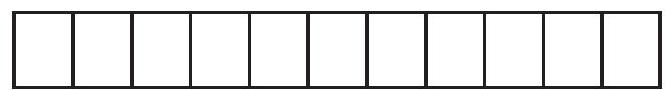
\includegraphics[max width=\textwidth, center]{2024_11_21_599d917d55a506aace4bg-01(1)}

PESEL ZDAJĄCEGO\\
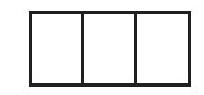
\includegraphics[max width=\textwidth, center]{2024_11_21_599d917d55a506aace4bg-01}

KOD\\
ZDAJĄCEGO

Arkusz opracowany przez Wydawnictwo Pedagogiczne OPERON.\\
Kopiowanie w całości lub we fragmentach bez zgody wydawcy zabronione.

\section*{ZADANIA ZAMKNIĘTE}
W zadaniach 1.-4. wybierz i zaznacz jedną poprawną odpowiedź.

\section*{Zadanie 1. (0-1)}
Wyrażenie \(\frac{\sqrt[3]{18}}{\sqrt[3]{9}-2 \sqrt[3]{3}+4}\) jest równe:\\
A. \(\sqrt[3]{36}-2 \sqrt[3]{18}\)\\
B. \(3 \sqrt[3]{2}+2 \sqrt[3]{18}\)\\
C. \(\frac{\sqrt[3]{54}-2 \sqrt[3]{18}}{7}\)\\
D. \(\frac{3 \sqrt[3]{2}+2 \sqrt[3]{18}}{11}\)

\section*{Zadanie 2. (0-1)}
Dany jest trapez \(A B C D\) w którym \(A B \| C D,|A B|=8,|C D|=3\). Na ramieniu \(B C\) zaznaczono punkt \(E\) w ten sposób, że \(\frac{|C E|}{|E B|}=\frac{1}{2}\). Przez punkt \(E\) poprowadzono prostą równoległą do \(A B\), która przecięła ramię \(A D\) w punkcie \(F\). Odcinek \(E F\) ma długość:\\
A. 3\\
B. \(4 \frac{2}{3}\)\\
C. \(5 \frac{1}{2}\)\\
D. 6

\section*{Zadanie 3. (0-1)}
Granica ciągu \(\lim _{n \rightarrow+\infty}\left(\sqrt{4 n^{2}+3 n}-2 n\right)\) jest równa:\\
A. 0\\
B. \(\frac{3}{4}\)\\
C. 1\\
D. \(+\infty\)

\section*{Zadanie 4. (0-1)}
Równanie \(\left|\frac{-4 x-17}{x+5}\right|=m\) ma dokładnie dwa rozwiązania dla:\\
A. \(m \in(-5,0) \cup(0,+\infty)\)\\
B. \(m \in(0,+\infty)\)\\
C. \(m \in(0,4) \cup(4,+\infty)\)\\
D. \(m \in(0,5) \cup(5,+\infty)\)

\section*{BRUDNOPIS (nie podlega ocenie)}
\begin{center}

\includegraphics[max width=\textwidth]{2024_11_21_599d917d55a506aace4bg-03}
\end{center}

\section*{ZADANIA OTWARTE}
\section*{Rozwiązania zadań 5.-15. należy zapisać w wyznaczonych miejscach pod treścią zadania.}
\section*{Zadanie 5. (0-2)}
Oblicz \(\log _{a b} \frac{\sqrt[3]{a}}{\sqrt{b}}\), jeżeli wiadomo, że \(\log _{a b} a=4\).\\
Zakoduj cyfrę jedności i dwie cyfry po przecinku otrzymanego wyniku.\\

\includegraphics[max width=\textwidth, center]{2024_11_21_599d917d55a506aace4bg-04}

\section*{Zadanie 6. (0-3)}
Znajdź równanie stycznej do wykresu funkcji \(f(x)=\frac{x-8}{4-3 x} \mathrm{w}\) punkcie \(\left(x_{0}, 3\right)\).

\begin{center}
\begin{tabular}{|c|c|c|c|c|c|c|c|c|c|c|c|c|c|c|c|c|c|c|c|c|c|c|c|c|c|c|c|c|c|}
\hline
 &  &  &  &  &  &  &  &  &  &  &  &  &  &  &  &  &  &  &  &  &  &  &  &  &  &  &  &  &  \\
\hline
 &  &  &  &  &  &  &  &  &  &  &  &  &  &  &  &  &  &  &  &  &  &  &  &  &  &  &  &  &  \\
\hline
 &  &  &  &  &  &  &  &  &  &  &  &  &  &  &  &  &  &  &  &  &  &  &  &  &  &  &  &  &  \\
\hline
 &  &  &  &  &  &  &  &  &  &  &  &  &  &  &  &  &  &  &  &  &  &  &  &  &  &  &  &  &  \\
\hline
 &  &  &  &  &  &  &  &  &  &  &  &  &  &  &  &  &  &  &  &  &  &  &  &  &  &  &  &  &  \\
\hline
 &  &  &  &  &  &  &  &  &  &  &  &  &  &  &  &  &  &  &  &  &  &  &  &  &  &  &  &  &  \\
\hline
 &  &  &  &  &  &  &  &  &  &  &  &  &  &  &  &  &  &  &  &  &  &  &  &  &  &  &  &  &  \\
\hline
 &  &  &  &  &  &  &  &  &  &  &  &  &  &  &  &  &  &  &  &  &  &  &  &  &  &  &  &  &  \\
\hline
 &  &  &  &  &  &  &  &  &  &  &  &  &  &  &  &  &  &  &  &  &  &  &  &  &  &  &  &  &  \\
\hline
 &  &  &  &  &  &  &  &  &  &  &  &  &  &  &  &  &  &  &  &  &  &  &  &  &  &  &  &  &  \\
\hline
 &  &  &  &  &  &  &  &  &  &  &  &  &  &  &  &  &  &  &  &  &  &  &  &  &  &  &  &  &  \\
\hline
 &  &  &  &  &  &  &  &  &  &  &  &  &  &  &  &  &  &  &  &  &  &  &  &  &  &  &  &  &  \\
\hline
 &  &  &  &  &  &  &  &  &  &  &  &  &  &  &  &  &  &  &  &  &  &  &  &  &  &  &  &  &  \\
\hline
\end{tabular}
\end{center}

Odpowiedź: \(\qquad\)

\section*{Zadanie 7. (0-3)}
Wykaż, że tylko jedna liczba spełnia nierówność \(\binom{n}{n-3} \leq n-1\).\\

\includegraphics[max width=\textwidth, center]{2024_11_21_599d917d55a506aace4bg-05}

\section*{Zadanie 8. (0-3)}
Dany jest trapez prostokątny o podstawach długości \(a, b\) oraz wysokości długości \(2 h\). Dłuższe ramię trapezu jest równocześnie średnicą okręgu, który jest styczny do drugiego ramienia trapezu. Udowodnij, że \(h^{2}=a b\).

\begin{center}
\begin{tabular}{|c|c|c|c|c|c|c|c|c|c|c|c|c|c|c|c|c|c|c|c|c|c|c|c|c|c|c|c|c|c|}
\hline
 &  &  &  &  &  &  &  &  &  &  &  &  &  &  &  &  &  &  &  &  &  &  &  &  &  &  &  &  &  \\
\hline
 &  &  &  &  &  &  &  &  &  &  &  &  &  &  &  &  &  &  &  &  &  &  &  &  &  &  &  &  &  \\
\hline
 &  &  &  &  &  &  &  &  &  &  &  &  &  &  &  &  &  &  &  &  &  &  &  &  &  &  &  &  &  \\
\hline
 &  &  &  &  &  &  &  &  &  &  &  &  &  &  &  &  &  &  &  &  &  &  &  &  &  &  &  &  &  \\
\hline
 &  &  &  &  &  &  &  &  &  &  &  &  &  &  &  &  &  &  &  &  &  &  &  &  &  &  &  &  &  \\
\hline
 &  &  &  &  &  &  &  &  &  &  &  &  &  &  &  &  &  &  &  &  &  &  &  &  &  &  &  &  &  \\
\hline
 &  &  &  &  &  &  &  &  &  &  &  &  &  &  &  &  &  &  &  &  &  &  &  &  &  &  &  &  &  \\
\hline
 &  &  &  &  &  &  &  &  &  &  &  &  &  &  &  &  &  &  &  &  &  &  &  &  &  &  &  &  &  \\
\hline
 &  &  &  &  &  &  &  &  &  &  &  &  &  &  &  &  &  &  &  &  &  &  &  &  &  &  &  &  &  \\
\hline
 &  &  &  &  &  &  &  &  &  &  &  &  &  &  &  &  &  &  &  &  &  &  &  &  &  &  &  &  &  \\
\hline
 &  &  &  &  &  &  &  &  &  &  &  &  &  &  &  &  &  &  &  &  &  &  &  &  &  &  &  &  &  \\
\hline
- &  &  &  &  &  &  &  &  &  &  &  &  &  &  &  &  &  &  &  &  &  &  &  &  &  &  &  &  &  \\
\hline
 &  &  &  &  &  &  &  &  &  &  &  &  &  &  &  &  &  &  &  &  &  &  &  &  &  &  &  &  &  \\
\hline
 & 到 &  &  &  &  &  &  &  &  &  &  &  &  &  &  &  &  &  &  &  &  &  &  &  &  &  &  &  &  \\
\hline
 &  &  &  &  &  &  &  &  &  &  &  &  &  &  &  &  &  &  &  &  &  &  &  &  &  &  &  &  &  \\
\hline
 & - &  &  &  &  &  &  &  &  &  &  &  &  &  &  &  &  &  &  &  &  &  &  &  &  &  &  &  &  \\
\hline
 &  &  &  &  &  &  &  &  &  &  &  &  &  &  &  &  &  &  &  &  &  &  &  &  &  &  &  &  &  \\
\hline
- &  &  &  &  &  &  &  &  &  &  &  &  &  &  &  &  &  &  &  &  &  &  &  &  &  &  &  &  &  \\
\hline
 & - &  &  &  &  &  &  &  &  &  &  &  &  &  &  &  &  &  &  &  &  &  &  &  &  &  &  &  &  \\
\hline
 &  &  &  &  &  &  &  &  &  &  &  &  &  &  &  &  &  &  &  &  &  &  &  &  &  &  &  &  &  \\
\hline
\end{tabular}
\end{center}

\section*{Zadanie 9. (0-4)}
W pudełku znajduje się 30 piłeczek ponumerowanych liczbami 1, 2, 3, 4, .., 30. Losujemy kolejno dwie piłeczki bez zwracania. Oblicz prawdopodobieństwo zdarzenia, że druga wylosowana piłeczka jest oznaczona liczbą pierwszą, jeżeli wiadomo, że pierwsza piłeczka była oznaczona liczbą nieparzystą. Wynik podaj w postaci nieskracalnego ułamka zwykłego.\\

\includegraphics[max width=\textwidth, center]{2024_11_21_599d917d55a506aace4bg-06(1)}

Odpowiedź: \(\qquad\)

\section*{Zadanie 10. (0-4)}
W trójkącie równobocznym \(A B C\) na boku \(A B\) zaznaczono punkt \(D\) w taki sposób, że \(\frac{|A D|}{|D B|}=\frac{1}{3}\).\\
Wyznacz sinus kąta \(B C D\).

\begin{center}
\begin{tabular}{|c|c|c|c|c|c|c|c|c|c|c|c|c|c|c|c|c|c|c|c|c|c|c|c|c|c|c|c|c|}
\hline
 &  &  &  &  &  &  &  &  &  &  &  &  &  &  &  &  &  &  &  &  &  &  &  &  &  &  &  &  \\
\hline
 &  &  &  &  &  &  &  &  &  &  &  &  &  &  &  &  &  &  &  &  &  &  &  &  &  &  &  &  \\
\hline
 &  &  &  &  &  &  &  &  &  &  &  &  &  &  &  &  &  &  &  &  &  &  &  &  &  &  &  &  \\
\hline
 &  &  &  &  &  &  &  &  &  &  &  &  &  &  &  &  &  &  &  &  &  &  &  &  &  &  &  &  \\
\hline
 &  &  &  &  &  &  &  &  &  &  &  &  &  &  &  &  &  &  &  &  &  &  &  &  &  &  &  &  \\
\hline
 &  &  &  &  &  &  &  &  &  &  &  &  &  &  &  &  &  &  &  &  &  &  &  &  &  &  &  &  \\
\hline
 &  &  &  &  &  &  &  &  &  &  &  &  &  &  &  &  &  &  &  &  &  &  &  &  &  &  &  &  \\
\hline
 &  &  &  &  &  &  &  &  &  &  &  &  &  &  &  &  &  &  &  &  &  &  &  &  &  &  &  &  \\
\hline
 &  &  &  &  &  &  &  &  &  &  &  &  &  &  &  &  &  &  &  &  &  &  &  &  &  &  &  &  \\
\hline
. &  &  &  &  &  &  &  &  &  &  &  &  &  &  &  &  &  &  &  &  &  &  &  &  &  &  &  &  \\
\hline
 &  &  &  &  &  &  &  &  &  &  &  &  &  &  &  &  &  &  &  &  &  &  &  &  &  &  &  &  \\
\hline
- &  &  &  &  &  &  &  &  &  &  &  &  &  &  &  &  &  &  &  &  &  &  &  &  &  &  &  &  \\
\hline
. &  &  &  &  &  &  &  &  &  &  &  &  &  &  &  &  &  &  &  &  &  &  &  &  &  &  &  &  \\
\hline
 &  &  &  &  &  &  &  &  &  &  &  &  &  &  &  &  &  &  &  &  &  &  &  &  &  &  &  &  \\
\hline
 &  &  &  &  &  &  &  &  &  &  &  &  &  &  &  &  &  &  &  &  &  &  &  &  & 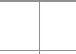
\includegraphics[max width=\textwidth]{2024_11_21_599d917d55a506aace4bg-06}
 &  &  &  \\
\hline
 &  &  &  &  &  &  &  &  &  &  &  &  &  &  &  &  &  &  &  &  &  &  &  &  &  &  &  &  \\
\hline
 &  &  &  &  &  &  &  &  &  &  &  &  &  &  &  &  &  &  &  &  &  &  &  &  &  &  &  &  \\
\hline
\end{tabular}
\end{center}

Odpowiedź: \(\qquad\)

\section*{Zadanie 11. (0-4)}
Rozwiąż równanie \(\sin ^{2} 2 x+1=7 \cos ^{2}\left(\frac{3}{2} \pi-x\right)\) dla \(x \in\langle-2 \pi, 2 \pi\rangle\).\\

\includegraphics[max width=\textwidth, center]{2024_11_21_599d917d55a506aace4bg-07}

Odpowiedź: \(\qquad\)

\section*{Zadanie 12. (0-6)}
Dla jakich wartości parametru \(m\) funkcje \(f(x)=\frac{4-m}{x}\) oraz \(g(x)=x^{2}+5 x+m\), dla \(x \neq 0\), mają dokładnie trzy punkty wspólne?\\

\includegraphics[max width=\textwidth, center]{2024_11_21_599d917d55a506aace4bg-07(1)}

Odpowiedź: \(\qquad\)

\section*{Zadanie 13. (0-4)}
Ciąg \(\left(a_{n}\right)\) jest ciągiem arytmetycznym. W wyniku podzielenia wyrazu \(a_{13}\) przez \(a_{3}\) otrzymujemy iloraz 5 i resztę 1, dodatkowo wyrazy pierwszy, siódmy i sto trzeci w podanej kolejności tworzą ciąg geometryczny. Oblicz iloraz ciągu geometrycznego.\\

\includegraphics[max width=\textwidth, center]{2024_11_21_599d917d55a506aace4bg-08}

Odpowiedź:\\
8

\section*{Zadanie 14. (0-6)}
Wyznacz równanie okręgu, który jest styczny do prostych \(x=0\) oraz \(4 x+3 y+33=0\), a także przechodzi przez punkt \(P(-2,0)\).\\

\includegraphics[max width=\textwidth, center]{2024_11_21_599d917d55a506aace4bg-09}

Odpowiedź: \(\qquad\)

\section*{Zadanie 15. (0-7)}
Obwód trójkąta równoramiennego jest równy L. Jakie długości powinny mieć boki tego trójkąta, aby objętość bryły powstałej w wyniku obrotu wzdłuż podstawy była największa?\\

\includegraphics[max width=\textwidth, center]{2024_11_21_599d917d55a506aace4bg-10}

Odpowiedź:\\
10

\section*{BRUDNOPIS (nie podlega ocenie)}

\includegraphics[max width=\textwidth, center]{2024_11_21_599d917d55a506aace4bg-11}\\

\includegraphics[max width=\textwidth, center]{2024_11_21_599d917d55a506aace4bg-12}


\end{document}